\documentclass[a4paper,14pt]{extreport}

%CONVENIENT COMMANDS
\newcommand{\bv}[1]{\hat{b_{#1}}}
\newcommand{\nv}[1]{\hat{n_{#1}}}

%PACKAGES
%Graphics
\usepackage{graphicx}
\graphicspath{ {./images/} }
%Math
\usepackage{amsmath}
\usepackage{bm}

%DOCUMENT START
\title{Attitude with an Attitude \\
\large An Informal Intro to Spacecraft Attitude Determination}
\author{Brian Leung\\University of Michigan, Class of 2022}

\begin{document}
\maketitle
\setcounter{tocdepth}{0}
\tableofcontents{}
\chapter{Preface}
\section{Prerequisites}
You're welcome to dive in and learn as you go, but knowing some \textbf{Physics 1/Dynamics} and \textbf{Linear Algebra} will help immensely. Honestly, with how applicable it is, you should just learn linear algebra in general. A class at the undergraduate level should more than enough. If you're dedicated enough, there's also plenty of online classes that you can take.

\section{Message to the Reader}
At the time of writing this, I am not a seasoned spacecraft engineer nor a cutting edge researcher (well, fingers crossed). For now, I'm just a green undergrad in Aerospace Engineering, hoping that my understanding  will help you out. I hope you learn something new and feel a little more comfortable in this field.

\section{Acknowledgement}
I owe much thanks to CU Boulder's ``Spacecraft Dynamics and Control Specialization" on Coursera, and Professor Hanspeter Schaub, the professor of the course. Seriously, it's great. If you've got the time and access, I highly recommend you look through it.

\section{What This Text Offers}
I really want to emphasize that this text is \underline{not} a university textbook level reference, bursting at the seams with advanced terminology and derivations. This will not delve into dynamic attitude determination or control theory either. 

This text is essentially CU Boulder's Specialization, Part 1, distilled down to the key takeaways. This will give you a quick and dirty intro to the fundamentals of spacecraft attitude description and determination, avoiding lengthy proofs and derivation. It offers conceptual questions along the way to test your knowledge. It can act as a springboard into more advanced topics for the aspiring spacecraft engineer.
\begin{center}
(TLDR: attitude determination speedrun any \% glhf)
\end{center}

\chapter{What is Attitude Anyways?}

\section{Definition}
Hint: It's not a state of mind. A fairly straightforward definition for attitude is:

\begin{center}
\textbf{ATTITUDE: A body's angular orientation with respect to a reference frame.}
\end{center}

A body just refers to something like a plane, spacecraft, or satellite. Angular orientation? Pretty self-explanatory. The important part of this definition is the reference frame. 

Let me pose this question to you. If you're floating around in an infinite black void, how do you decide which way is up? or down? Of course, the problem is a bit more complex than that, but it's a question you can't answer without the help of a \textit{reference frame}.

\subsection{Frames?}

When I say reference frame, or frames in general, I mean coordinate frames: XYZ, \(\hat{i}\hat{j}\hat{k}\), 3 basis vectors, etc. You can pretty much glue a coordinate frame onto anything your heart desires. Attaching frames to things helps ground them in a mathematical context, and that helps in more reasons than I can name. For example, it's a lot easier to say things like "I'm about 10 meters south and 1 meter east of you with respect to your NED frame". This is just a rough example, but there are plenty of other good reasons to put frames on bodies.

\begin{center}
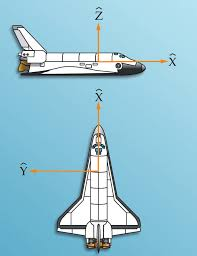
\includegraphics[width=4cm]{shuttle_body_frame}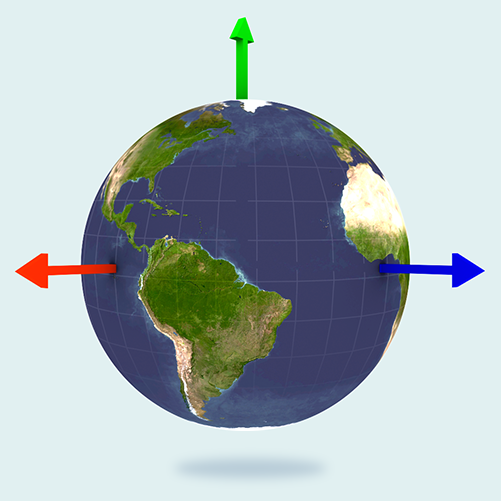
\includegraphics[height=5.2cm]{ecef}\\
A Frame on the Space Shuttle (L) \\ ECEF (Earth Centered, Earth Fixed) Frame (R)
\end{center}
\textbf{BODY: Refers to object of interest (e.g. spacecraft, satellite)}\\
When someone says "Body Frame" that refers to the frame glued to your satellite, space shuttle, UFO, rover. Basically, the thing you're trying to keep track of.\\\\
\textbf{INERTIAL: Refers to reference (e.g. Earth)}\\
When someone says inertial frame, they always mean reference. In most basic problems, the Earth and its variety of frames is what you'll refer to as inertial. However, you can also set the inertial frame to something that's not the Earth, like the ISS.\\

\subsection{It's All Relative}
I must emphasize that \emph{attitude is all relative}. Without knowing and specifying a reference frame, the description of your attitude is basically useless. 

\subsection{Why Worry About Attitude Anyways?}
Trying to brush off attitude determination as unimportant is similar to asking "Why do planes have to be headed in the right direction?". Depending on the project/mission, the importance of making sure your object is pointed in the desired direction ranges anywhere from marginal (super basic cubesats) or critical (space telescopes, comms satellites, space shuttle). But 9 times out of 10, attitude is pretty high on the priority list. This topic also has plenty of applications outside of the aero sphere, such as in video games, robotics, and biomechanics.

\section{4 Basic Truths}
\begin{enumerate}
\item \textbf{You need a minimum of 3 coordinates to describe relative angular displacement in 3D.} There's likely some in-depth proof showing why this is the case, but I'm not qualified enough to comment on it. The best example of a 3 coordinate set is Euler Angles, covered in Ch 4.

\item \textbf{A 3 coordinate set will have at least 1 geometric orientation where the coordinates are \underline{singular}.} When an attitude description becomes \textbf{singular}, it's best described as acting ... weird. As in, the math doesn't behave very nicely (divisions by 0, non-uniqueness, etc.). As a real life example, think gimbal lock. The gimbal, when turned a certain way, loses degrees of freedom.

\item \textbf{At/near the singularities, the kinematic differential equations are also singular.} When you get close to a singularity in your attitude description, the kinematic differential equations of your attitude description also turn feral. These won't be too heavily covered in this text so don't worry too much about them.

\item \textbf{Redundant sets of 4 or more coordinates exist that are universally valid.}

\end{enumerate}
\chapter{DCM}
\section{Definitions and Things}
It doesn't stand for dichloromethane. And please, don't call it a DCM matrix.

\begin{center}
\textbf{DIRECTION COSINE MATRIX: A transformation matrix that converts from one reference frame to another.}
\end{center}

We consider the DCM the ``mother of all attitude parameterizations", quoting Professor Schaub. When I mean \emph{attitude parameterization}, I mean descriptions of your attitude, such as quaternions, Euler angles, etc. Every DCM maps to a parameterization of your choice and every parameterization maps back to a DCM. You could say it's the center of the great web of parameterizations. With DCMs, we directly interact with the basis vectors of the frames themselves. Before we move any further, let's get some \emph{formalisms} out of the way.
\subsection{Funky Formalisms}
When describing the body frame, I'll use the letter b. Describing the basis vectors that make up the body frame, I'll say $\bv{1}, \bv{2}, \bv{3}$. Likewise, describing the inertial frame basis vectors uses the letter n, like so: $\nv{1}, \nv{2}, \nv{3}$. Constantly writing out $\bv{1}, \bv{2}, \bv{3}$ is gonna get old real fast, so lets save our hands some work and assemble them into something called a \emph{vectrix}.
\[
\{\hat{b}\} = 
\begin{bmatrix}
\bv{1}\\ \bv{2}\\ \bv{3}\\
\end{bmatrix}\;
\{\hat{n}\} = 
\begin{bmatrix}
\nv{1}\\ \nv{2}\\ \nv{3}\\
\end{bmatrix}
\] 

In addition to saving ink, vectrices are also easier to do linear algebra with, since they're (for all intents and purposes) matrices. When the time comes, I'll refer to the components of a matrix, like so:
\[
[C] = \begin{bmatrix}
C_{11}&C_{12}&C_{13}\\
C_{21}&C_{22}&C_{23}\\
C_{31}&C_{32}&C_{33}
\end{bmatrix}\
\]

Pretty standard matrix stuff. Now, we can get into the math.
\section{The Math: A Tale of 2 Frames}
Here's a diagram of the 2 frames. $\bv{1}$ forms angles $\alpha_{11}, \alpha_{12}, \alpha_{13}$ with the 3 inertial basis vectors $\nv{1},\nv{2},\nv{3}$. This applies for the other body vectors as well, but that's just not shown on the diagram.
\begin{center}
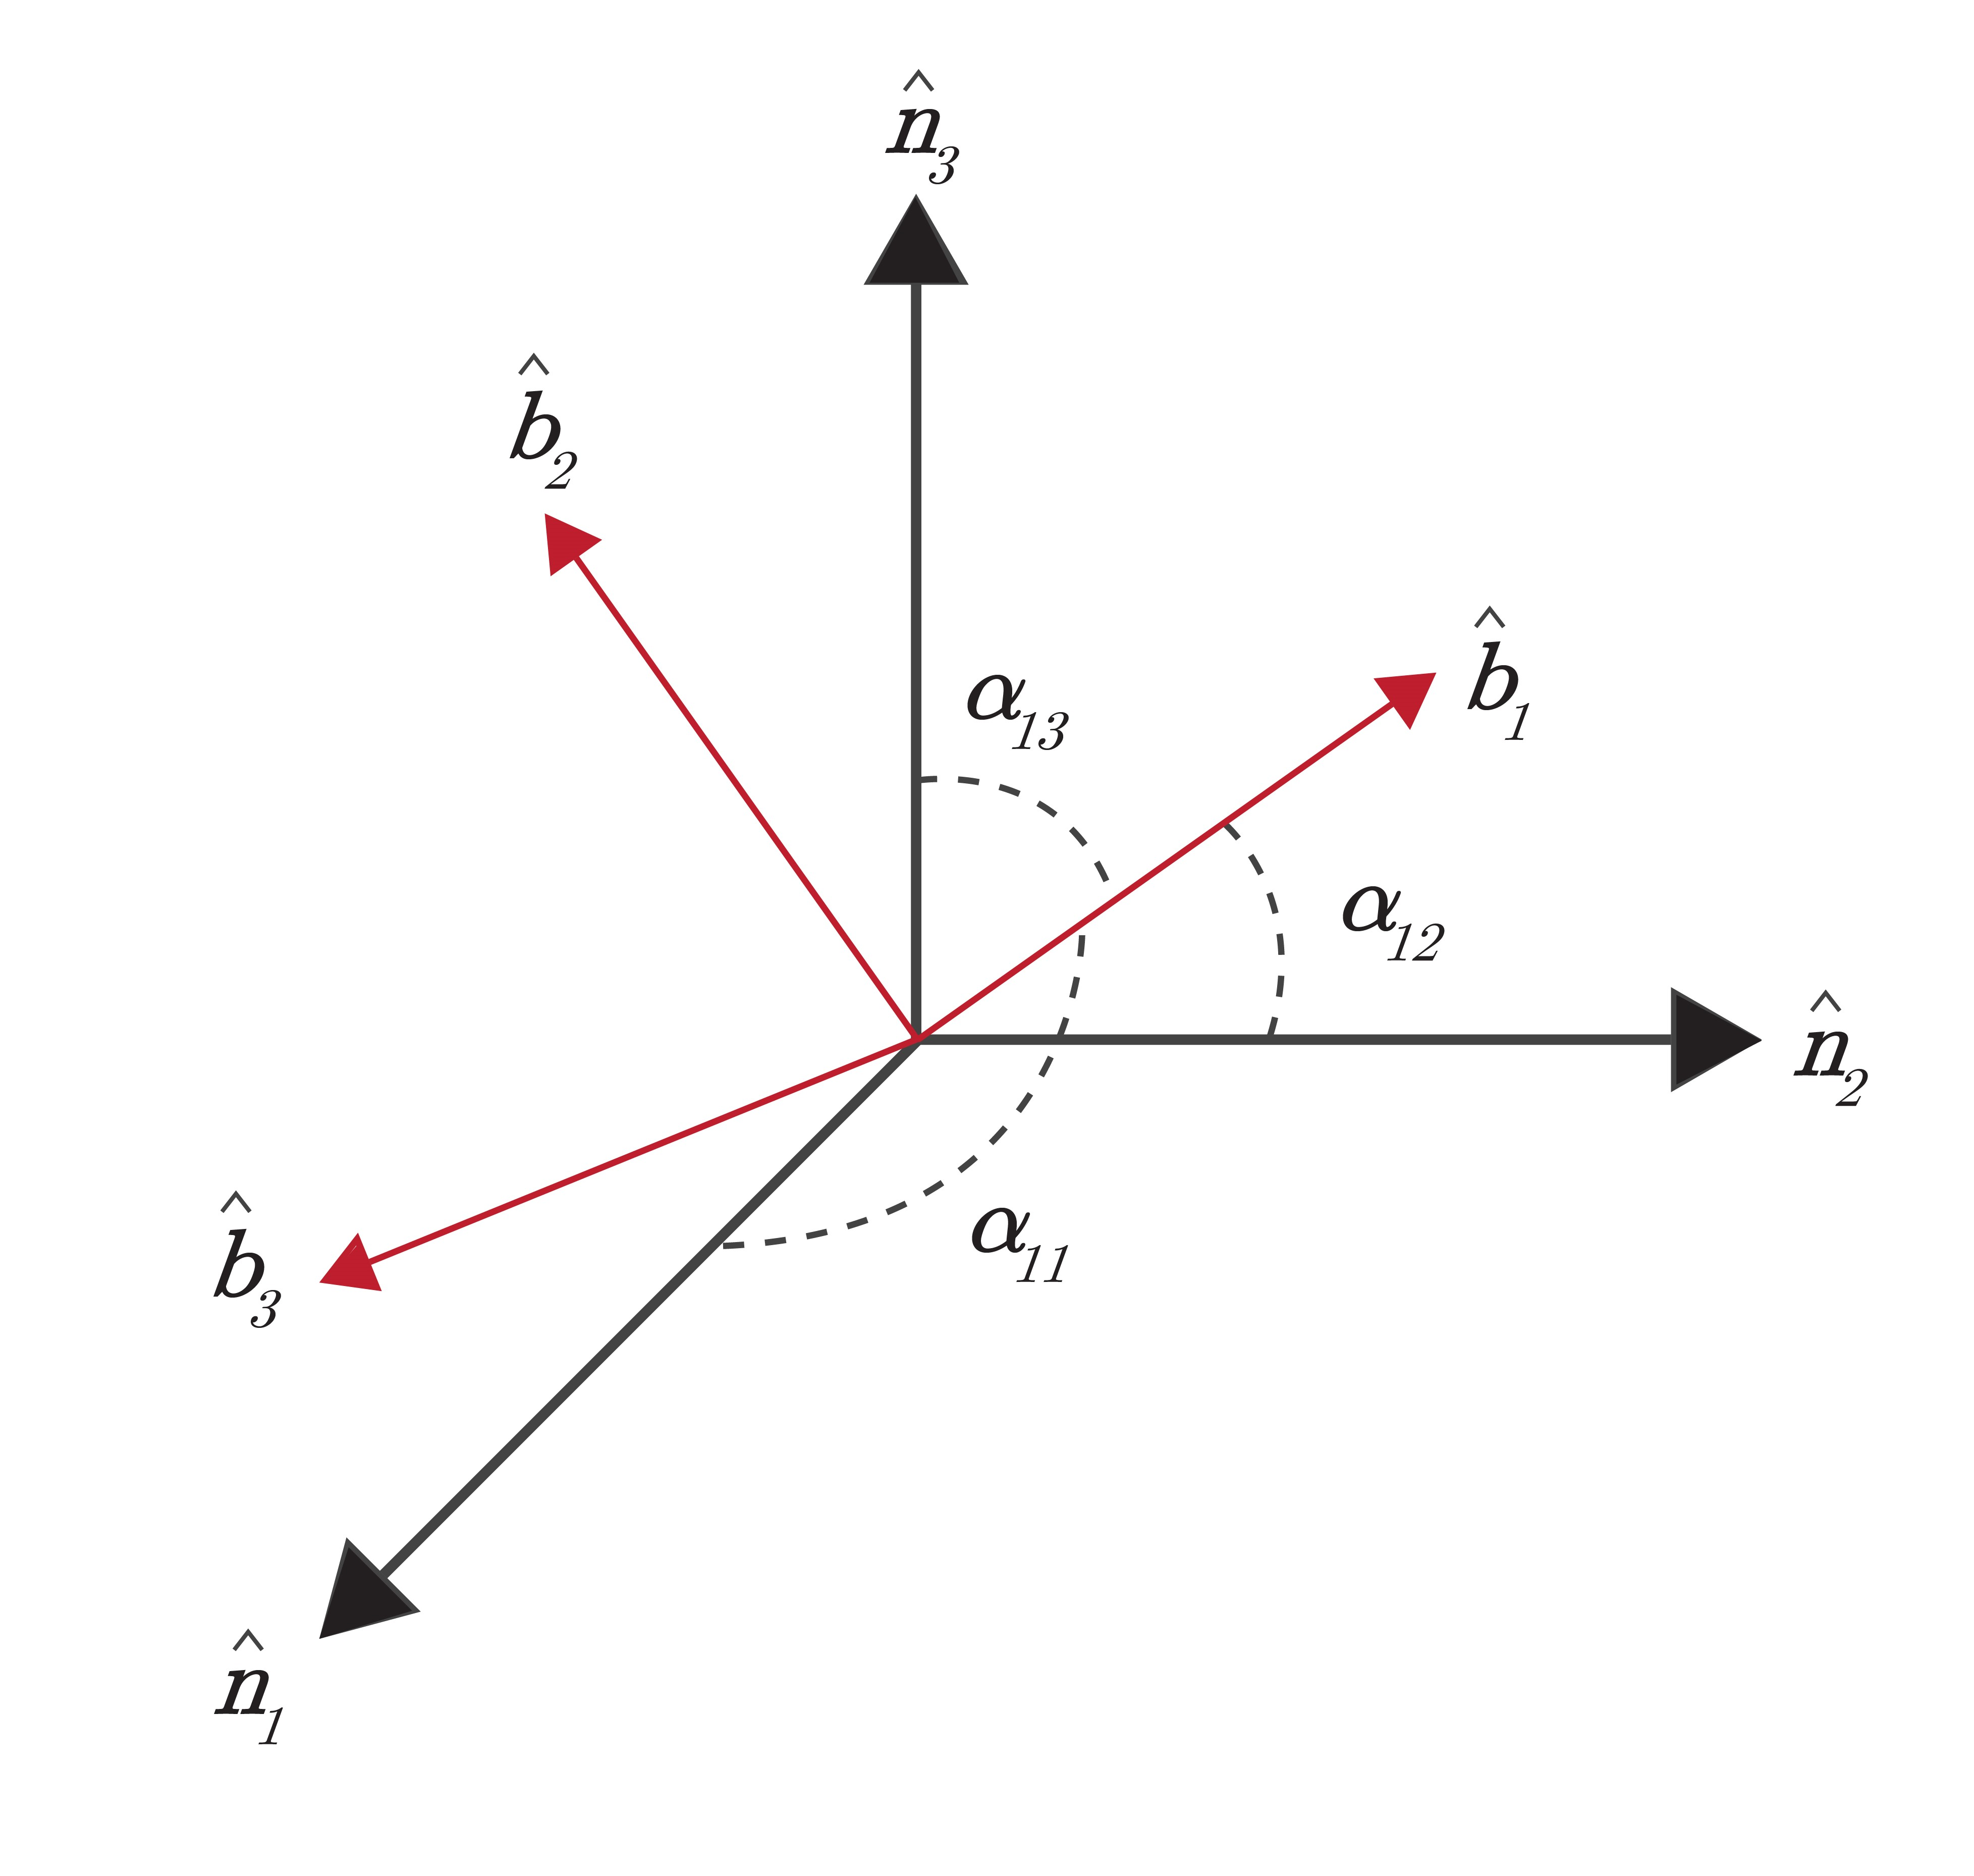
\includegraphics[width=7cm]{dcmalpha}
\end{center}
A good way to relate a body frame vectors to an inertial frame vectors is via the following:

\[\bv{1} = \cos(\alpha_{11})\nv{1} + \cos(\alpha_{12})\nv{2} + \cos(\alpha_{13})\nv{3}\]
\[\bv{2} = \cos(\alpha_{21})\nv{1} + \cos(\alpha_{22})\nv{2} + \cos(\alpha_{23})\nv{3}\]
\[\bv{3} = \cos(\alpha_{31})\nv{1} + \cos(\alpha_{32})\nv{2} + \cos(\alpha_{33})\nv{3}\]
\\
The cosines find the projection of each $\hat{b}$ against each $\hat{n}$. Being masters of linear algebra, we can immediately organize this whole thing into the following, to convert from inertial to body frame:

\[
\{\hat{b}\} = \begin{bmatrix}
\cos(\alpha_{11})&\cos(\alpha_{12})&\cos(\alpha_{13}) \\
\cos(\alpha_{21})&\cos(\alpha_{22})&\cos(\alpha_{23}) \\
\cos(\alpha_{31})&\cos(\alpha_{32})&\cos(\alpha_{33})
\end{bmatrix} \{\hat{n}\} = [BN] \{\hat{n}\}
\]
And from the definition of a cosine, we can also say:
\[
\{\hat{b}\} = \begin{bmatrix}
b_1 \cdot n_1 & b_1 \cdot n_2 & b_1 \cdot n_3 \\
b_2 \cdot n_1 & b_2 \cdot n_2 & b_2 \cdot n_3 \\
b_3 \cdot n_1 & b_3 \cdot n_2 & b_3 \cdot n_3
\end{bmatrix} \{\hat{n}\} = [BN] \{\hat{n}\}
\]
We'll call this matrix [BN]. The BN matrix we have here is the \emph{Direction Cosine Matrix}. It doesn't take a rocket scientiest to see that the ``Direction Cosine" part of the name comes from all these cosines. DCMs are basically glorified rotation matrices.
\subsection{Well, Whats The Point?}
Glad you asked. Here's a situation: You are on Earth and your friend is on a spaceship in orbit. You just saw a really cool star and want to radio up to your friend where to look, with respect to their frame. You know the DCM that converts from your frame to theirs. How would you achieve this?

If it wasn't obvious, it's via that DCM you have. Lets say that v is the vector to the star. We can describe it in both the inertial frame and body frame, like so:
\[v = v_{b1}\bv{1}+v_{b2}\bv{2}+v_{b3}\bv{3}=[v_b]^T\{\hat{b}\}\;(1)\]
\[v = v_{b1}\nv{1}+v_{n2}\nv{2}+v_{n3}\nv{3}=[v_n]^T\{\hat{n}\}\;(2)\]
The $[v_b]$ and $[v_n]$ just indicate the coefficients that you multiply your basis vectors by. That T in the right side of the equation just indicates a transpose. All in all, real standard coordinate frame stuff. 

Well, we have that \{b\} vectrix in the equation 1 and we know that $\{\hat{b}\} = [BN]\{\hat{n}\}$. So lets get to substituting.
\[[v_b]^T\{\hat{b}\} = [v_n]^T\{\hat{n}\}\]
\[[v_b]^T[BN]\{\hat{n}\} = [v_n]^T\{\hat{n}\}\]
Doing some funky transposing and linear algebra things, we'll discover that:
\[\bm{v_b = [BN]v_n}\]
and likewise,
\[\bm{v_n = [BN]^Tv_b}\]
As you can see, DCMs not only \emph{help describe how one frame is rotated relative to another}, but it can also help \emph{translate what one vector looks like to an observer in a different frame}.
\section{Adding and Subtracting DCMs}
Despite all we've been doing so far, we are allowed to have more than 2 frames. For example, let's say your UFO is floating outside the ISS. You know the DCM that converts the ISS frame to your UFO frame. You also know the DCM that converts some inertial frame to ISS frame. What if you want to know how to convert from inertial straight to UFO frame? 

Lets represent the UFO frame as U, the ISS frame as I, and the inertial frame to N. We want to find the DCM [UN], but we only know [UI] and [IN]. The solution is super simple:
\[\bm{[UN] = [UI][IN]}\]

This is what we call \emph{DCM Addition.} But what about \emph{DCM Subtraction}?

Let's say we already know [UN] and we know [IN]. How would we find the UFO frame relative to the ISS frame [UI]? Following our addition we can say:
\[[UI] = [UN][NI]\]
But wait a second, we don't know [NI]? We actually do. Transposing an orthogonal matrix gives the inverse.
\[[IN]^T = [NI]\]
Thus we can say:
\[\bm{[UI] = [UN][IN]^T}\]
Doing this to [UN] subtracts out the part where I is related to N.
\section{Properties}
Well, what makes a DCM a DCM?
\begin{enumerate}
\item{\textbf{DCMs are 3x3}}

\item{\textbf{The magnitude of each row and column is 1.}}

Ensuring the rows and columns are unit length makes the math less chaotic. Let's say that some malevolent DCM doesn't maintain unit length. When you multiply some vector through this DCM, the vector that comes out on the other side isn't the same length as the original. And now, not only do you have to keep track of a ton of numbers, you have to scale that vector's components up or down. Since we want to make our lives as easy as possible, this ain't the move.

\item{\textbf{Every DCM element is $\leq |1|$}}

A consequence of the above. Not exactly hard to see why.

\item{\textbf{DCMs are orthogonal}}

Using vetrices with orthogonal vectors is convention because they're mathematically friendly. The fact that a DCM is orthogonal is the reason we can use the transpose to transform backwards from body to inertial. The inverse of an orthogonal matrix is just its transpose after all.

\item{\textbf{The determinant of a DCM is $1$ (Unit, Orthogonal, and Right Handed)}}

This property is essentially a result of the previous properties piled together. A unit orthogonal matrix has a determinant of $\pm 1$. Why $\pm 1$ you ask? Well the sign of the determinant indicates the handedness of the DCM. A +1 indicates a right handed frame and -1 is a left handed frame. A left handed frame technicallyyyyy isn't wrong, but right handed frames are convention. For the sake of consistency, let's just say DCMs are right handed.

\item{\textbf{DCMs are non-singular!}}

There's no divisions by zero, no weird functions, and since we're working at the lowest level, not many ambiguities can arise.
\end{enumerate}

\subsection{Wait a minute...}
If DCMs are non-singular, why don't we exclusively use them to describe attitude? While DCMs are great and non-singular, they're not always the easiest/intuitive paramaterization to use. 


The sheer amount of elements in the DCM is not very convenient. 9 elements to keep track of attitude? With properties that we constantly have to enforce? Tacking on angular velocity $\omega$ and multiple frames, the amount of numbers flying around can quickly get out of hand.

DCMs aren't super easy to visualize. If I hand you a list of 9 numbers, would you be able to immediately tell how the body frame is rotated? Probably not.

However, the DCM is super useful for translating between attitude parameterizations.

\section{Test Your Knowledge}
\begin{enumerate}
\item Identify the illegal DCMs:\\\\
	$
	a.
	\begin{bmatrix}
			1&0&0\\
			1&0&0\\
			0&1&0
	\end{bmatrix} 
	b.	
	\begin{bmatrix}
			2&0&0\\
			0&2&0\\
			0&0&2
	\end{bmatrix}
	c.	
	\begin{bmatrix}
			1&0&0\\
			0&0.866&-0.5\\
			0&0.5&0.866
	\end{bmatrix}
	d.
	\begin{bmatrix}
			-1&0&0\\
			0&-1&0\\
			0&0&1
	\end{bmatrix}$ 
\item{Given DCMs [KB], [KJ], [NJ], how would you find DCM [BN]?}
\end{enumerate}

\chapter{Euler Angles}

\section{Definitions and Things}

If you've heard of yaw pitch or roll, you've most certainly heard of Euler Angles.
\begin{center}
\textbf{EULER ANGLES: A parameterization that describes attitude in 3 sequential rotations.}
\end{center}

The definition is pretty self explanatory. To describe an attitude in Euler angles, you need to specify your type of Euler angle, referred to as a \emph{set}. Then, you specify the degrees of the angles that belong to this set. Each of the angles describe how far you rotate the frame around that specified axis. 

Here's a visual example if it ain't too clear:

\begin{center}
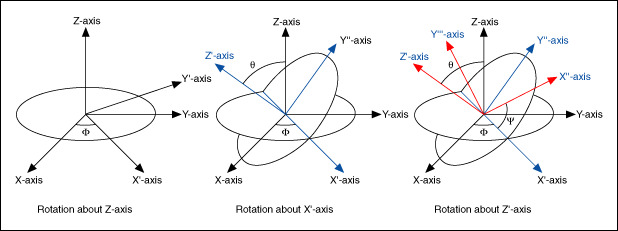
\includegraphics[width=16cm]{euler_proper}
\end{center}

This is what's described as a 3-1-3 Euler Angle, since the rotations operate on the Z, X, and Z body axes. The rotation sequence does the following:
\begin{enumerate}
\item Rotate the frame around the Z-axis by angle $\phi$. This forms a new frame with $X'$ and $Y'$ axes.
\item Rotate the frame around the X' axes by angle $\theta$. This forms a frame with the $Z'$ and $Y''$ axes.
\item Finally, rotate the frame around the Z' axis by angle $\psi$. This forms a frame with the $X''$ and $Y'''$ axes, and the rotation is finished.
\end{enumerate}

Of course, this is not the only set out there.

\section{Types of Euler Angles}
Euler angles fall into two categories.

\begin{enumerate}
\item{\textbf{Symmetric:}

A Symmetric Euler set implies that the first and last rotation axes are repeated. The best example of this is the 3-1-3 Euler angle shown above.}

\item{\textbf{Asymmetric:}

On the other hand, Asymmetric Euler sets don't have repeating rotation axes. You're probably most familiar with the Yaw-Pitch-Roll or 3-2-1 set.}
\end{enumerate}

In total, there are 12 possible sets.
\section{Euler Angles to DCMs}
Euler Angles relate to DCMs pretty seamlessly. We can represent each individual rotation around an axis as a DCM. These individual rotations just move us from intermediate frame to intermediate frame. Once you have all these DCMs together, you can just multiply them together to find the overall DCM. 

But how do we represent rotations around axes as DCMs?:
\begin{center}
Rotation around axis 1 (X):
\[[R_1(\theta)] = \begin{bmatrix}
			1&0&0\\
			0&\cos{\theta}&\sin{\theta}\\
			0&-\sin{\theta}&\cos{\theta}
	\end{bmatrix}\]	
Rotation around axis 2 (Y):
\[[R_2(\theta)] = \begin{bmatrix}
		\cos{\theta}&0&-\sin{\theta}\\
		0&1&0\\
		\sin{\theta}&0&\cos{\theta}
	\end{bmatrix}\]
Rotation around axis 3 (Z):
\[[R_3(\theta)] = \begin{bmatrix}
		\cos{\theta}&\sin{\theta}&0\\
		-\sin{\theta}&\cos{\theta}&0\\
		0&0&1
	\end{bmatrix}\]

To get the full DCM of a $\alpha\beta\gamma$ Euler set:
\[[BN(\theta_1,\theta_2,\theta_3)] = [R_\gamma(\theta_3)][R_\beta(\theta_2)][R_\alpha(\theta_1)]\]
\end{center}
(Depending who you work with, $\theta_1,\theta_2,\theta_3$ is the same as $\phi,\theta,\psi$, respectively. It'll vary with who you ask, just make sure you clarify.)
\section{DCMs to Euler Angles}
Converting from DCMs to Euler Angles is a little more complex. 
\section{Singularities}

\section{Test Your Knowledge}

\chapter{Principal Rotation Vectors}
\section{Definitions and Things}

Euler Angles are great, but you \emph{really} don't wanna use them for spacecraft and other body frames that can tumble head over heels. Moving away from the world of Euler angles, let's try something new. 

First, a theorem for us to internalize. Known as \emph{Euler's Principal Rotation Theorem}, it states that:

\begin{center}
\textbf{THEOREM: A rigid body can be brought from a start to an end orientation by a single rigid rotation ($\phi$ rad/deg) around some principal axis ($\hat{e}$). This principal axis is fixed in both the start and end orientation.}
\end{center}

\begin{center}
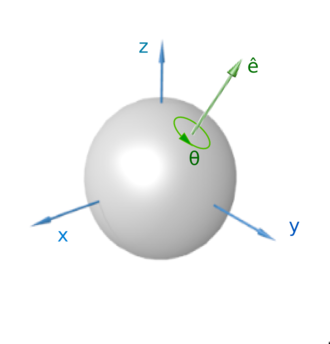
\includegraphics[width=8cm]{PRV1}

(I know it says $\theta$, just pretend it's $\phi$)
\end{center}

We can take advantage of this theorem and extract the \textbf{Principal Rotation Vector} parameterization, also known as \emph{PRVs} for short.\\

PRVs consist of 2 parts:
\begin{enumerate}
\item{\textbf{$\mathbf{\hat{e}}$, The Principal Rotation Vector}

As the name may have revealed, you indeed need to define a principal rotation vector to spin your frame around. The components of the principal rotation vector are labeled as $\mathbf{<e_1, e_2, e_3>}$ }

\item{$\mathbf{\phi}$, \textbf{How Far to Rotate}

You also need to define how far to spin the frame around the PRV.}
\end{enumerate}

\section{PRVs to DCM}
This section isn't too complex, the formula is just thick.
\[[BN] = \begin{bmatrix}
			e_1^2\Sigma+c_\phi&e_1 e_2 \Sigma + e_3 s_\phi&e_1 e_3 \Sigma - e_2 s_\phi\\
			e_2 e_1 \Sigma - e_3 s_\phi&e_2^2 \Sigma + c_\phi&e_2 e_3 \Sigma + e_1 s_\phi\\
			e_3 e_1 \Sigma + e_2 s_\phi&e_3 e_2 \Sigma - e_1 s_\phi&e_3^3 \Sigma + c_\phi
	\end{bmatrix}\]	
\[
\Sigma = 1-c_\phi
\]
Note that the $c_\phi,s_\phi$ are just shorthand for $\cos{\phi},\sin{\phi}$
\section{DCM to PRVs}
Thankfully, this process is a little slimmer.

\[
cos(\phi) = \dfrac{1}{2}(C_{11}+C_{22}+C_{33}-1)
\]
\[
\hat{e} = \begin{bmatrix}
e_1\\e_2\\e_3\\
\end{bmatrix} = \dfrac{1}{2\sin{\phi}}
\begin{bmatrix}
C_{23}-C_{32}\\C_{31}-C_{13}\\C_{12}-C_{21}\\
\end{bmatrix}
\]
\chapter{The Quaternion}
Googling ``quaternion math" will probably scare you, unless you're a math major. Taken in the context of PRVs however, they're actually pretty straightforward. They're probably one of the most popular non-singular attitude descriptors out there. 

Just to get this out of the way, you'll probably hear the term ``Euler Parameters" being used (EPs for short) and you might wonder what the difference is. Quaternions are the mathematical construct and Euler Parameters are the \emph{coefficients} of the quaternion. 
 
\subsection{Well, what is a quaternion?}
Quaternions form a number system that extends the complex number system. It was invented by William Rowan Hamilton back in 1843, after having an epiphany on a bridge near his home in Ireland. They're usually represented with 4 terms:
\[
a + bi + cj + dk
\]
Where a,b,c,d are the real coefficients and i,j,k well... aren't. I'm not gonna go too in the weeds with this since I'm not qualified enough to say more.

\chapter{Attitude Determination?}
Now that you got a good chunk of the preliminaries out of the way, let's get into how it's applied. The whole idea of \emph{Attitude Determination} is broken up into 2 types of problems:
\begin{enumerate}
\item{
\textbf{Static Attitude Determination:} You take all of your measurements at the same time, and try to solve for the optimal geometry of the measurements, figuring out your attitude at that instant of time.
}
\item{\textbf{Dynamic Attitude Determination:} You take your measurements over time and try to figure out how your body is spinning around. This is a far harder problem and one that this text will not cover.
}
\end{enumerate}


\chapter{TRIAD Method}
Published in 1964, TRIAD is one of the oldest algorithms out there. Despite its age, it is still a viable method for simpler satellites.
\chapter{Wahba's Problem}
TRIAD is great and all, but what if we want to make use of all the sensors we have on our satellite? After all, your sponsor would probably be pissed if they paid for a GPS receiver and 4 star trackers but you're only using 1 star tracker and a sun sensor.
\chapter{Davenport's Q}

\chapter{QUEST}
Davenport's Q is lovely, but computationally, solving that eigenvector problem is pretty expensive.
\chapter{Answer Key}
\section{Chapter 1 DCM}
\begin{enumerate}
\item{a \& b}
\item{$[KB]^T[KJ][NJ]^T$}
\end{enumerate}
\end{document}